
\section{Introdução} \label{sec:Introdução}

Os microsserviços são a abordagem principal para a construção de sistemas nativos da nuvem. A arquitetura de microsserviços (MSA) prescreve que um sistema compreende serviços implementáveis de forma independente que interagem
% com um objetivo mais centralizado de criar um conjunto de tecnologia
\cite{lewis2014microservices}. Um microsserviço deve ter uma única responsabilidade, o que significa que eles gerenciam apenas uma parte específica das necessidades da organização. Os microsserviços permitem a evolução descentralizada de partes do sistema e sua escalabilidade seletiva.
% Um benefício dos microsserviços é que cada parte específica do sistema pode ser facilmente compreendida e aplicada a outros sistemas de software e projetos \cite{thones2015microservices}. Os microsserviços podem ser implementados usando contêineres ou por meio de processos individuais.
A criação de um serviço baseado em MSA ajuda a eliminar a dependência de determinadas tecnologias, permitindo que os usuários acessem a infraestrutura específica do serviço \cite{cerny2018contextual}. No entanto, os microsserviços são desenvolvidos e evoluídos por equipes independentes e descentralizadas, apesar do resultado que os usuários veem como um produto holístico.

Garantir que o sistema geral funcione adequadamente, independentemente de suas dependências internas e decomposição, é vital. Com a complexidade cada vez maior do sistema e especialmente quando descentralizado, é importante buscar a cobertura completa do sistema, o que muitas vezes é difícil de conseguir. Mas só então poderíamos descobrir se todas as funções do sistema são avaliadas para entradas adequadas e impróprias.

Juntamente com o teste funcional, é vital avaliar se o sistema responde adequadamente a várias quantidades de usuários e solicitações em carga simultânea. Esse teste de carga pode acompanhar os testes funcionais enquanto monitora os tempos de resposta do sistema.

%O termo 'carga' neste caso refere-se à taxa ou número de usuários e solicitações acessando o sistema fornecido \cite{jiang2008automatic}. O teste de carga ajuda a garantir que as ações do usuário no sistema sejam estáveis, avaliando como o sistema reage a várias quantidades de carga. Existem três maneiras principais de executar o teste de carga. Essas técnicas de geração de carga incluem a utilização de usuários reais para gerar a carga, usando drivers de carga ou implantando os testes de carga em plataformas especiais \cite{jiang2015survey}. Avaliar o comportamento de um sistema em várias quantidades de carga pode destacar áreas de melhoria, como gargalos ou áreas de falha no sistema. Esses problemas geralmente só podem ser descobertos usando o teste de carga porque eles ocorrem ou são visíveis apenas sob uma certa quantidade de carga no sistema.

% Também é importante garantir que um sistema mantenha sua qualidade visual em vários navegadores. Websites\todo{ser sistemas de uso consistente e não websites} são distribuídos através do modelo de arquitetura cliente-servidor \cite{cross_browser_testing}, de modo que indivíduos de qualquer lugar do mundo possam acessá-los usando qualquer número de navegadores diferentes. Vários navegadores possuem seu próprio método de interpretação de documentos HTML e, como resultado, possuem seu próprio método de renderização de HTML na tela \cite{peachpit}. Embora existam ferramentas que ajudarão na padronização do HTML, os desenvolvedores de sites ainda devem realizar testes de navegador da web. O teste do navegador da Web ajudará a garantir a qualidade dos sites e manter sua visualização em vários navegadores da Web \cite{smartbear_cross_browser_testing}.

Considerando os testes funcionais e de carga, identificamos que a comunidade de microsserviços está perdendo um benchmark de conjunto de testes que poderia ser usado para novos avanços e evolução da pesquisa neste campo. Devido a essa falta, elaboramos um estudo de caso para mostrar nosso progresso na geração desse benchmark.

O objetivo central de nossa contribuição é fornecer à comunidade científica um conjunto de testes abrangente para dois sistemas de microsserviços bem estabelecidos. Especificamente, estamos focando este trabalho em testes funcionais e de carga. Esses tipos de teste são uma parte importante do teste da funcionalidade geral desses sistemas.

Apresentamos os benchmarks do conjunto de testes por meio de um estudo de caso. Também identificamos e discutimos vários desafios que surgiram ao testar esses sistemas e apresentamos algumas das melhores práticas e correções para problemas comuns. Desenvolvemos um conjunto completo de testes de ``melhor esforço" que abrange os pontos de extremidade dos vários microsserviços em cada sistema. O conjunto de testes pode ser usado por pesquisadores para validar seu trabalho em testes de microsserviços em um conjunto de testes comum.

As demais seções estão organizadas da seguinte forma. A Seção 2 fornece informações sobre os microsserviços e ferramentas. A Seção 3 cobre nosso estudo de caso seguido pelo benchmark apresentado na Seção 4. A Seção 5 conclui o artigo.

\section{Background}\label{sec:fundo}

\todo[inline]{Timmy nota 5/31 Precisamos explicar isso com tantos detalhes, ou podemos assumir um certo nível de conhecimento. Parece-me que toda esta seção do preâmbulo poderia ser condensada em uma frase por parágrafo e presa em diferentes subseções.}

\todo[inline]{TOMAS, precisamos de cortes drásticos. \\Sugiro condensar introdução + A + B em um único parágrafo \\ benchmarks do sistema são bons}

\todo[inline]{TOMAS, precisamos selecionar cada palavra com cuidado e podemos remover as coisas que são texto desnecessário enquanto mantemos a mensagem e bom entendimento para os leitores;\\talvez possamos reduzir ``Facing Initial Pitfalls"}

O teste funcional garante que vários recursos do sistema funcionem de acordo com as especificações ou expectativas da funcionalidade do sistema. Os casos de teste normalmente são baseados nas especificações dos componentes de software e cada teste corresponde a um determinado requisito ou recurso de software. Isso ajuda a garantir que as partes do conjunto geral de software funcionem de forma independente. O foco nos requisitos de software garante que a saída seja consistente com as expectativas do usuário final.

Para simular a interação do usuário com sistemas de microsserviços, consideramos o sistema como uma caixa preta e usamos suas interfaces de usuário sem saber detalhes internos. Para auxiliar nesses testes, vários frameworks trazem a capacidade de projetar scripts de teste. Por exemplo, a estrutura do Selenium facilita o teste do sistema da web. Ele fornece um método de navegadores da Web automatizados que acionam eventos como se os usuários os tivessem feito.

O teste de regressão funcional verifica o sistema após a modificação, garantindo que todos os recursos, fluxos e funcionalidades do sistema estejam funcionando como na versão anterior ou por uma especificação ou expectativa de funcionalidade correta. Ele ajuda na garantia de qualidade do sistema e ajuda a evitar mudanças não intencionais no sistema causadas por mudanças apressadas.

O % Selenium permite que os testadores criem scripts para testes de navegador da Web em várias linguagens com suporte, como Ruby, Java, Python e C\#. O WebDriver do Selenium executa scripts para navegadores específicos \cite{browserStack_selenium}. Ele fornece uma API, biblioteca, driver e estrutura para os testadores escreverem e executarem seus scripts de teste.

Além da funcionalidade, também é importante analisar como um sistema se comporta durante várias condições de carga.
O teste de carga é o processo de simulação da demanda do sistema que testa o comportamento sob várias condições. O termo 'carga' neste caso refere-se à taxa ou número de usuários e requisições acessando o determinado sistema \cite{jiang2008automatic}. O teste de carga ajuda a garantir que as ações do usuário no sistema sejam estáveis, avaliando como o sistema reage a várias quantidades de carga.

Existem três maneiras principais de executar o teste de carga. Essas técnicas de geração de carga incluem a utilização de usuários reais para gerar a carga, usando drivers de carga ou implantando os testes de carga em plataformas especiais \cite{jiang2015survey}. Avaliar o comportamento de um sistema em várias quantidades de carga pode destacar áreas de melhoria, como gargalos ou áreas de falha no sistema. Esses problemas geralmente só podem ser descobertos usando o teste de carga porque eles ocorrem ou são visíveis apenas sob uma certa quantidade de carga no sistema.

Da mesma forma, existem estruturas que podem ajudar na automação de testes. Por exemplo, Gatling \cite{gatling} pode executar um script de teste e gerar relatórios de carga abrangentes.

% O teste de carga pode destacar os principais locais de um determinado sistema que causam gargalos ou falhas para os usuários. Em sua essência, o teste de carga ajuda a garantir que o sistema atenda aos requisitos de desempenho pretendidos, geralmente identificados em um contrato de nível de serviço (SLA).

Outra métrica importante no teste de software é a cobertura do teste. Ajuda a medir a quantidade de testes feitos em um determinado sistema. A cobertura dos testes mostra quais partes do sistema estão sendo executadas ao longo dos testes, medida por uma razão entre o número de elementos particulares do sistema cobertos pelos testes e o número total desses elementos no sistema. %Um conjunto completo de testes de cobertura executa todas as partes do sistema testado.


% \subsection{Teste de regressão funcional}\label{sec:functional}

% O teste funcional procura estabelecer se cada recurso do sistema funciona de acordo com os requisitos do sistema; considera que a saída é consistente com as expectativas do usuário final.

% O teste de regressão funcional verifica o sistema depois que a modificação é aplicada ou novos recursos são adicionados ao sistema. Ele verifica se todos os recursos, fluxos e funcionalidades do sistema estão funcionando como na versão anterior, ou por especificação ou expectativa de uma funcionalidade correta. Ele ajuda na garantia de qualidade do sistema e ajuda a evitar mudanças não intencionais no sistema causadas por mudanças apressadas.

% Para simular a interação do usuário com sistemas de microsserviços, consideramos o sistema como uma caixa preta e usamos suas interfaces de usuário. Para ajudar com esses testes, existem estruturas de teste que trazem a capacidade de criar scripts de teste.

% Por exemplo, a estrutura do Selenium facilita o teste automatizado do sistema da web. O Selenium fornece um método de navegadores da Web automatizados que acionam eventos como se fossem feitos pelos usuários. O Selenium permite que os testadores criem scripts para teste de navegador da Web em várias linguagens com suporte, como Ruby, Java, Python e C\#. O WebDriver do Selenium executa scripts para navegadores específicos \cite{browserStack_selenium}. Ele fornece uma API, biblioteca, driver e estrutura para os testadores escreverem e executarem seus scripts de teste.


% \subsection{Teste de carga}

% Um exemplo de ferramenta de teste de carga é o Gatling. % (versão 3.9.2). Utilizamos esta ferramenta por ser uma ferramenta amplamente utilizada e de fácil acesso. Como esta ferramenta é de código aberto, todos os recursos são fornecidos ao usuário gratuitamente.
% O Gatling utiliza principalmente dois componentes centrais: o registrador Gatling e o mecanismo Gatling. O gravador é capaz de gerar scripts com base em um arquivo HAR (HTTP Archive) ou por meio de um proxy HTTP. O mecanismo Gatling executa um determinado script de teste e gera um relatório que consiste em arquivos HTML. Existem três linguagens principais nas quais os testes em Gatling podem ser escritos: Scala, Java ou Kotlin \cite{gatling}.
% % Decidimos usar Scala por ser a linguagem mais usada para esta ferramenta.

% % \subsection{Reconstrução de processos de negócios}

% A reconstrução do processo de negócios está usando logs de rastreamento obtidos durante o teste para criar uma visão geral dos microsserviços usados e as interações entre eles para um caso de uso específico. Isso pode ser usado para ajudar usuários não técnicos a entender as interações de nível de serviço que entram em cada caso de uso, bem como a ordem e a frequência em que são chamadas.

% Essa reconstrução do processo de negócios também pode ser usada como uma validação dos vários cenários ou casos de uso testados. A partir de nossos testes, podemos delinear os endpoints e microsserviços específicos que devem ser atingidos durante a execução. Podemos então comparar esses resultados com a reconstrução do processo de negócios gerada a partir dos logs de rastreamento. Isso adiciona outra etapa para ajudar a validar nossos resultados. Exemplos de reconstrução baseada em processos de negócios foram propostos por Taibi e Systa~\cite{Taibi2019}, com o objetivo de decompor sistemas monolíticos em microsserviços. No entanto, eles não consideraram questões de teste.

\subsection{Referências do sistema de microsserviços}
\label{subsec:benchmark}

Para demonstrar testes funcionais e de carga para microsserviços, foram utilizados dois sistemas bem estabelecidos e baseados na comunidade que fornecem uma ampla gama de funcionalidades que podem ser testadas ao longo de um estudo de caso. O Train-Ticket \cite{trainticket} é baseado na plataforma Java, e o eShopOnContainers \cite{eshop} usa C\#. Essa seleção de sistema nos permite ilustrar diferentes cenários em nosso estudo de caso, resultando em um benchmark de teste compartilhável para esses sistemas.

% \subsubsection{Microsserviço de Bilhete de Trem}
% \label{subsec:train}

{\bf The Train-Ticket benchmark} fornece um sistema de reserva de bilhetes de trem baseado em 47 microsserviços (a partir da versão 1.0.0). A figura \ref{fig:train} mostra o layout geral e a estrutura da arquitetura Train-Ticket. Ele mostra como o front-end, o sistema de monitoramento e os serviços interagem dentro do sistema. Essa figura permite que os usuários entendam como cada um dos microsserviços do sistema Train-Ticket depende um do outro.

\todo[inline]{Sheldon (6/1): Os comentários em nosso artigo mencionavam que as figuras 1 e 2 eram difíceis de ler. Como devemos consertar isso?}

\begin{figura}[h]
     \centering
     \hspace{-1.3em}
     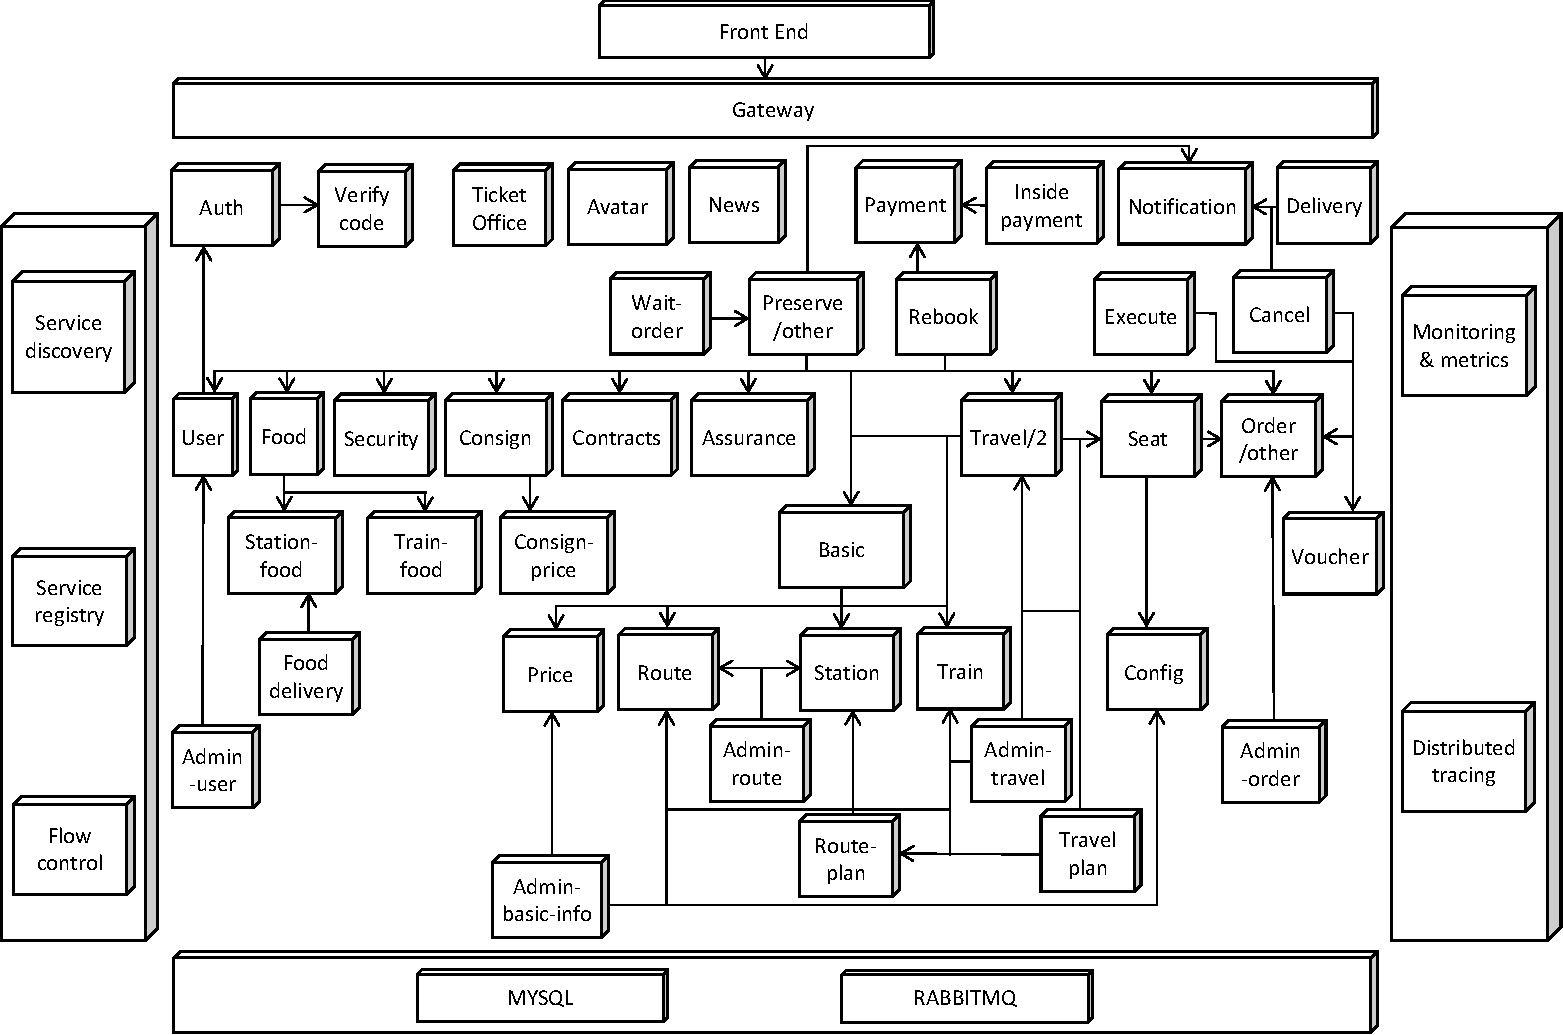
\includegraphics[width=1.02\columnwidth]{img/trainticket-our.pdf}
     % \vespaço{-0,4cm}
        \caption{Arquitetura do Bilhete de Trem \cite{bilhete de trem}}
     % \vespaço{-0,7cm}
        \label{fig:trem}
\end{figura}

Os casos de uso envolvidos com este sistema de microsserviço podem ser divididos em ações de usuário e administrador. Certas ações estão presentes para todos os usuários, como o sistema de login, enquanto outras dependem do tipo de usuário.

Existem seis casos de uso \texttt{usuário} principais dentro do sistema Train-Ticket. Esses casos são a procura de um trem, a reserva de uma passagem, a atualização da consignação, o pagamento da passagem, a retirada da passagem e a entrada na estação.

Os casos de uso do \texttt{admin} envolvem a adição, atualização e exclusão de vários elementos do sistema de emissão de bilhetes, como pedidos, rotas, planos de viagem, usuários, contatos, estações, trens, preços e configurações.

Para nosso estudo de caso, estamos usando a versão 1.0.0 do Train-Ticket, lançada em 9 de agosto de 2022 \cite{trainticket}. Este sistema de microsserviço foi criado pela Fudan University CodeWisdom Team. O objetivo original desse sistema era fornecer um sistema de referência para bilhetagem ferroviária \cite{zhou2018benchmarking}.

Este sistema foi criado usando uma infinidade de diferentes linguagens de programação e frameworks como Java (Spring Boot, Spring Cloud), Node.js (Express), Python (Django), Go (Webgo) e MongoDB e MySQL para os bancos de dados \cite {Bilhete de trem}.

% \subsubsection{eShopOnContainers Microservice}

{\bf O sistema de microsserviço eShopOnContainers} é um exemplo de aplicativo de referência .Net Core \cite{eshop}. O sistema está centrado em fornecer vários casos de uso envolvidos em aplicativos de compras eletrônicas. O front-end para este microsserviço é dividido entre dois aplicativos da web: um aplicativo da web tradicional feito com HTML e um aplicativo de página única (SPA) feito com typescript e Angular 2. Há também um componente de aplicativo móvel para esse sistema de microsserviço.

A arquitetura desse aplicativo é multiplataforma no servidor e no lado do cliente. A figura \ref{fig:eshop} mostra um layout da interação entre os aplicativos cliente e o host Docker. Dentro do host Docker, existem vários microsserviços autônomos com cada serviço contendo seus próprios dados ou banco de dados. Diferentes abordagens para a estrutura dos microsserviços são utilizadas, como padrões CRUD e DDD/CQRS. HTTP é a principal forma de comunicação entre esses microsserviços e os aplicativos clientes com os quais o usuário interage \cite{eshop}.

\begin{figura}[h]
     \centering
     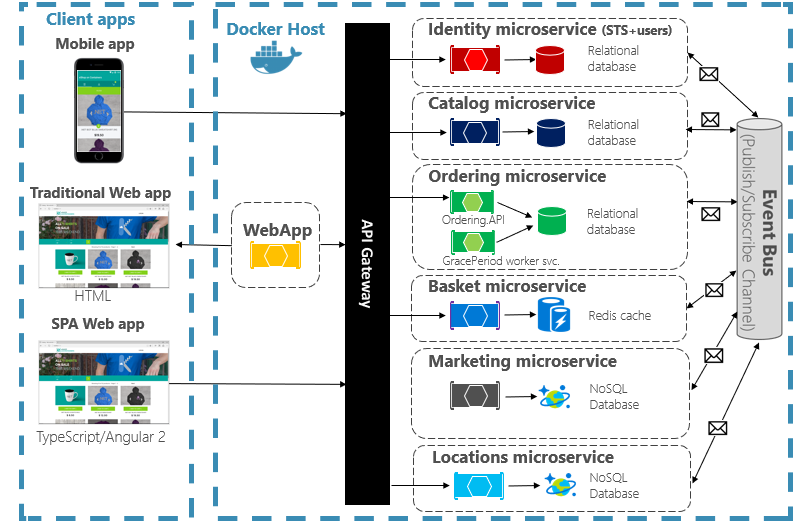
\includegraphics[width=\columnwidth]{img/eshop-architecture-2.png}
     % \vespaço{-0,4cm}
        \caption{arquitetura eShopOnContainers \cite{eshop}}
     % \vespaço{-0,7cm}
        \label{fig:eshop}
\end{figura}

Há uma infinidade de casos de uso que o usuário pode executar neste aplicativo. Para interagir ao máximo com a funcionalidade, o usuário deve fazer login com a conta de demonstração pré-criada ou pode registrar uma nova conta no sistema. Um usuário pode filtrar os itens com base em vários campos, o que não depende do login do usuário no sistema. Um \texttt{usuário registrado} pode adicionar itens ao carrinho, que podem ser atualizados na página do carrinho. Os usuários podem concluir o processo de checkout para finalizar o pedido ou cancelar o pedido. Por fim, os usuários podem visualizar os pedidos anteriores que concluíram.

  Para nosso estudo de caso, usamos a versão 5.0.0 do microsserviço eShopOnContainers. Este sistema de microsserviço é fornecido como um dos aplicativos de referência pela .NET Application Architecture \cite{eshop}; além disso, possui amplas contribuições da comunidade em seu repositório de código-base.

% \section{Trabalhos Relacionados}
% \label{sec:relacionado}

% \todo[inline]{Timmy note 5/31 Eu diria para despejar esta seção de trabalho relacionada, parece

\section{Estudo de caso}\label{sec:use_case}

O objetivo do nosso estudo de caso é criar um conjunto abrangente de testes centrados na funcionalidade de todos os endpoints do sistema, de modo a avaliar o sistema e sua funcionalidade sob estresse e determinar o comportamento de sistemas de microsserviços bem estabelecidos.


Como estamos nos concentrando em testes funcionais e de carga para nosso estudo de caso, nosso benchmark de teste está centrado na avaliação do tempo de resposta das ações, na interação da interface do usuário e na funcionalidade geral do sistema.

O teste de funcionalidade considera o sistema como uma caixa preta e desconhece a decomposição interna para microsserviços, que muitas vezes reflete a visão do usuário. O benchmark de teste de interface do usuário (baseado na web) ajuda a garantir a consistência durante a execução das ações do usuário.

O teste de funcionalidade por meio da interface do usuário garante que o sistema exiba as informações de maneira correta e consistente. Se houver variabilidade nas informações exibidas, isso poderá afetar muito a experiência do usuário.

O teste de carga visa identificar possíveis locais de gargalo e lentidão. Isso é importante porque a experiência do usuário pode ser significativamente afetada por esses problemas. No entanto, com o teste de carga, podemos considerar o sistema como uma caixa cinza e focar nos endpoints expostos ao middleware.


% Existem muitas facetas do teste funcional, mas para nosso estudo de caso, focamos no teste de carregamento e do navegador da web.

Como mencionado anteriormente, os sistemas de microsserviços de teste de carga são vitais para garantir que os vários microsserviços reajam bem a diferentes quantidades de carga. Isso pode ajudar a identificar áreas de gargalos e falhas no sistema.


Ao longo do processo de nosso estudo de caso, vários desafios surgiram ao testar esses sistemas de microsserviços. Neste estudo de caso, apresentaremos algumas das melhores práticas e correções para problemas comuns que podem surgir durante o teste.

\subsection{Estudo de caso de teste de regressão funcional}

Queríamos garantir a exatidão da funcionalidade fornecida pelo sistema de microsserviço implementando um conjunto de testes automatizado baseado na Web. Usamos o Selenium para essa finalidade e conseguimos garantir que os microsserviços funcionem e sejam exibidos corretamente em vários ambientes de navegador. Queríamos garantir a implementação de testes automatizados para testar minuciosamente a funcionalidade e o design dos microsserviços. Para este estudo de caso, nosso objetivo foi fornecer um conjunto de testes completo que inclui testes funcionais e de interface do usuário para simular de perto a experiência de um usuário ao utilizar os sistemas de microsserviços.

Usamos o framework Selenium para escrever testes automatizados que simulavam a experiência de um usuário dos sistemas de microsserviços Train-Ticket e eShopOnContainers.

% Ao longo deste processo, nos deparamos com muitos desafios e obstáculos, que queremos destacar juntamente com nosso processo de desenvolvimento do conjunto de testes do Selenium.

\subsubsection{Desenho do Estudo}
Primeiro, criamos manualmente uma lista abrangente de casos de uso em cada microsserviço. Nossa abordagem para criar uma lista de casos de uso abrangentes foi registrar todas as ações possíveis que o usuário poderia realizar ao interagir com o microsserviço e testar o resultado dessa ação. Acompanhamos os casos de uso em uma planilha e marcamos cada caso de uso à medida que o teste automatizado foi concluído. Manter uma lista de casos de teste nos ajudou a acompanhar quais casos de uso foram totalmente testados e forneceu um bom indicador de nosso progresso até a cobertura total. Este documento foi compartilhado junto com nosso benchmark de teste no Zenodo \cite{zenodo_benchmark}.

\subsubsection{Procedimento do Estudo / Enfrentando as Armadilhas Iniciais}
Descartamos o Katalon Web Recorder \cite{katalon}, pois os scripts resultantes continham muitos códigos não modularizados, repetitivos e ilegíveis. Prosseguimos manualmente com nossos próprios scripts Selenium. Executáveis como testes JUnit para nosso teste automatizado de navegador da web, testaríamos nosso trabalho usando um navegador da web Chrome. Esse navegador da Web nos permitiu visualizar como nosso código interagia com os microsserviços e nos permitiu interromper a execução e inspecionar o navegador da Web durante a depuração. Embora o uso de um navegador da web Chrome seja bom para depurar e escrever os testes, usar esse método não é eficiente ao executar vários testes, pois vários navegadores da web são gerados para cada teste e sobrecarregam a tela.

Agrupamos casos de uso semelhantes em testes para reduzir o número de testes executados. Agrupar os testes ajudou a reduzir etapas redundantes e aumentou a eficiência. Após a criação dos testes, em vez de executá-los no navegador Chrome, passamos a executar os testes no HTML Unit WebDriver, que é um driver da Web sem GUI. Ele suporta JavaScript e simulará um navegador da Web para testes com outros frameworks, como JUnit \cite{html_unit}. Isso também acelerou o tempo de processamento de nossos testes JUnit. No entanto, queríamos tornar nossos testes ainda mais eficientes, paralelizando~os.

Utilizamos o framework TestNG com a capacidade de paralelizar os testes \cite{testng}. Além disso, o TestNG permite que o testador tenha mais controle sobre os testes e é capaz de especificar o número de threads em que os testes serão executados. Passamos do uso do JUnit como nossa estrutura de teste para o uso do TestNG. Após a troca de frameworks, paralelizamos nossos testes para torná-los mais eficientes. Após a paralelização dos testes do Selenium, agora o tempo necessário para executá-los foi reduzido drasticamente.

\subsubsection{Resultados do Estudo}
\todo[inline]{Timmy nota 5/31 Não sou um grande fã de todas essas grandes tabelas de coisas, só porque não acho que elas necessariamente transmitam algo crucial.}
\todo[inline]{Tomas eu ficaria com eles, me parecem interessantes se eu quiser usar o benchmark}
  %\todo[inline]{Cerny TODO: Atualizamos esta seção}
  %\todo[inline]{Tomas: Eu poderia estar interessado em saber quantos testes únicos existem, talvez uma tabela com totais por projeto e tipo de teste Scala/Selenium}
  %\todo[inline]{Resolvido, verifique a tabela abaixo e nos avise se houver algum comentário}

Como nosso procedimento era criar um conjunto abrangente de testes da funcionalidade fornecida pelo usuário, nosso objetivo era interagir com todas as funcionalidades possíveis expostas ao usuário para melhor simular a experiência do usuário. Como resultado do nosso estudo de caso de regressão funcional, acabamos testando um total de 51 casos de uso para o sistema TrainTicket e um total de 26 casos de uso para o sistema eShopOnContainers, conforme mostrado na Tabela \ref{tab:selenium-test-count }.

\begin{tabela}[h]
    \centering
    \begin{tabular}{|P{4cm}|P{4cm}|}
    \hline
        \textbf{Conjunto de testes} e \textbf{\# de casos de uso do Selenium}\\
    \hline \hline
        Admin TrainTicket & 33\\
        Cliente TrainTicket & 18\\
    \hline
        \textbf{Combined TrainTicket} & \textbf{51}\\
    \hline
        \textbf{eShopOnContainers} & \textbf{26}\\
   
    \hline
    \end{tabular}
    \caption{Número de testes de Selenium por Suite\\Use Case Benchmark}
    \label{tab:selenium-test-count}
\mesa final}

 Embora tenhamos nos esforçado para implementar totalmente todos os casos de uso possíveis, havia um caso de uso no sistema de microsserviço TrainTicket que não pudemos testar totalmente, que era o serviço de consignação. Embora tenhamos escrito completamente o teste para o serviço de remessa, não conseguimos implantar esse serviço no sistema TrainTicket. Portanto, nosso teste funcionaria teoricamente, mas não conseguimos verificar seus resultados.

O conjunto de teste de reserva TrainTicket abrange todos os casos de uso do lado do cliente, devido à sua co-dependência um do outro. O conjunto de teste de reserva envolve o uso do recurso de pesquisa regular para localizar e reservar uma passagem, pagar pela passagem, alterar a ordem da passagem, coletar a passagem e entrar na estação. O conjunto de teste de reserva também inclui o uso do recurso de pesquisa avançada para encontrar e reservar um segundo bilhete, cancelar esse bilhete e, finalmente, excluir todas as informações adicionadas no final do teste. Todos esses casos de uso são ações que um cliente normalmente realizaria ao reservar e gerenciar seu bilhete.

\begin{comentário}
 \begin{tabela}[h]
    \centering
    \begin{tabular}{|P{4cm}|P{2,5cm}|}
    \hline
        Conjunto de testes e nome do teste\\
    \hline\hline
        & ConfigLista\\
        & Lista de contatos\\
        & Conecte-se\\
        Lista de & Pedidos\\
        Admin & Lista de Preços\\
        & ListadeRotas\\
        & StationList\\
        & TrainList\\
        & TravelList\\
        & Lista de usuários\\
    \hline
        Cliente & Reservas\\
        & Conecte-se\\
    \hline
    \end{tabular}
    \caption{Nome dos testes TrainTicket Selenium\\Use Case Benchmark}
    \label{tab:selenium-trainticket-test-name}
\mesa final}
\end{comentário}

\início{tabela}[h]
\centering
\begin{tabular}{|P{1cm}|P{2cm}|P{4,5cm}|}
\hline
\textbf{Conjunto de Testes} & \textbf{Teste} & \textbf{Casos de Uso}\\
\hline \hline
\multirow{6}{*} & \multirow{2}{*}{Login do cliente} & Login válido/inválido,\\
                         & & Usuário/Senha inválido, Sair\\
                         \cline{2-3}
                         & \multirow{4}{*}{Reservas} & Reservar Econômica, Reservar Primeira Classe,\\
                         & & Criar/Salvar Contato,\\
  Cliente & & Reserve com Garantia, com Refeições,\\
                         & & com Consignar, Cancelar\\
                         \cline{2-3}
                         & \multirow{2}{*}{Lista de pedidos} & Número de telefone inválido,\\
                         & & Atualizar Consignar, Pagar pelo Bilhete\\
                         \cline{2-3}
                         & Recolher Bilhete & Recolher Bilhete\\
                         \cline{2-3}
                         & Entrar na Estação & Entrar na Estação\\
                         \cline{1-3}
                         & \multirow{2}{*}{Login do administrador} & Login válido/inválido,\\
                         & & Usuário/Senha inválido, Sair\\
                         \cline{2-3}
                         & Lista de Pedidos & Adicionar/Atualizar/Excluir Pedido\\
                         \cline{2-3}
                         & Lista de Rotas & Adicionar/Atualizar/Excluir Rota\\
                         \cline{2-3}
                         & Lista de Viagens & Adicionar/Atualizar/Excluir Viagem\\
                         \cline{2-3}
                         & Lista de Usuários & Adicionar/Atualizar/Excluir Usuário\\
                         \cline{2-3}
  Administrador e lista de contatos e adicionar/atualizar/excluir contato\\
                         \cline{2-3}
                         & Lista de Estações & Adicionar/Atualizar/Excluir Estação\\
                         \cline{2-3}
                         & Lista de Trens & Adicionar/Atualizar/Excluir Trem\\
                         \cline{2-3}
                         & Lista de Preços & Adicionar/Atualizar/Excluir Preço\\
                         \cline{2-3}
                         & Lista de Configuração & Adicionar/Atualizar/Excluir Configuração\\
\hline
\end{tabular}
\caption{Nome dos testes TrainTicket Selenium\\Use Case Benchmark}
\label{tab:selenium-trainticket-test-name-new}
\vespaço{-1em}
\mesa final}

O conjunto de teste de checkout eShopOnContainers envolve preencher o carrinho com um item, navegar até a tela de checkout e verificar se o sistema precisa das informações formatadas para prosseguir com o checkout e fazer o pedido.

\begin{tabela}[!t]
\centering
\begin{tabular}{|P{2,5cm}|P{5,5cm}|}
\hline
\textbf{Teste} & \textbf{Casos de Uso}\\
\hline \hline
  \multirow{3}{*} & Login válido/inválido,\\
     Login e usuário/senha inválidos,\\
                         & Sair\\
  \cline{1-2}
  \hline
  \multirow{6}{*}{Registro} e credenciais válidas/inválidas,\\
                         & Credenciais ausentes,\\
                         & Nome de usuário único,\\
                         & Senhas Correspondentes,\\
                         & Data de Expiração Inválida,\\
                         & Conecte-se\\
  \cline{1-2}
  \hline
  \multirow{2}{*}{Navegar nas páginas} e Próxima página,\\
                         & Página anterior\\
  \cline{1-2}
  \hline
  \multirow{3}{*}{Pesquisa/Filtragem} e pesquisa por marcas,\\
                         & Pesquisar por tipos,\\
                         & Pesquisa em vários campos\\
\cline{1-2}
  \hline
  \multirow{3}{*}{Atualizar Carrinho} e Incrementar Carrinho (Salvar/Não Salvar),\\
                         & Diminuir Carrinho (Salvar/Não Salvar),\\
                         & Remover item\\
  \cline{1-2}
  \hline
  \multirow{2}{*}{Checkout} & População de informações,\\
                         & Check-out válido/inválido\\
\hline
\end{tabular}
\caption{Nome do eShopOnContainers Selenium Tests\\Use Case Benchmark}
\label{tab:selenium-eshoponcontainers-test-name-new}
\vespaço{-2em}
\mesa final}

%\todo[inline]{Tabela 4 é o que tenho até agora, tenho que me afastar um pouco, mas poderia substituir a Tabela 2 acima?}

Tabela \ref{tab:selenium-trainticket-test-name-new} e Tabela \ref{tab:selenium-eshoponcontainers-test-name-new} lista todos os testes TrainTicket e eShopOnContainers Selenium. O número de testes para TrainTicket e eShopOnContainers é muito menor do que a quantidade de casos de uso que abrange cada microsserviço, conforme descrito na Tabela I. Como agrupamos casos de uso semelhantes, acabamos com muito menos testes do que casos de uso.

A paralelização das suítes de teste eShopOnContainers resultou em uma execução mais rápida dos testes. Antes de paralelizar nossos testes de regressão funcional, observamos que o tempo de execução seria em média de 25 segundos. Depois de implementarmos o Html Unit e a estrutura de teste TestNG, observamos que o tempo de execução seria em média de 6 a 7 segundos, que foi o tempo de execução do teste mais lento.

Embora nossos testes ainda sejam relativamente pequenos em tamanho, nosso estudo de caso é uma evidência de que a paralelização de testes de regressão funcional economiza tempo, especialmente para projetos maiores e conjuntos de testes.

\subsection{Teste de Carga}

Em nosso estudo de caso de teste de carga, queríamos nos concentrar em testar o tempo de resposta dos vários endpoints nos sistemas de microsserviços. Mais especificamente, queríamos fornecer testes para que a comunidade pudesse ver como esses microsserviços respondem a uma variedade de cargas diferentes. Procuramos oferecer aos interessados uma forma de visualizar os diversos problemas que podem surgir à medida que mais usuários acessam o sistema. Isso inclui ver os possíveis gargalos e o tempo de resposta do sistema.

Conforme elaborado em segundo plano, usamos Gatling (versão 3.9.2) para criar nossos testes de carga para ambos os sistemas. Nas próximas seções, mostraremos nosso processo para projetar e implementar testes baseados em carga enquanto trabalhamos para obter uma lista abrangente de testes avaliando os endpoints em cada microsserviço.

% Ao testar esses sistemas, identificamos alguns obstáculos ao implementarmos certas áreas de nossos testes. Este estudo de caso também serve para mostrar nosso processo de avaliação e resolução de vários tipos de problemas que podem ocorrer. Destacamos esses desafios e as formas de prevenir ou mitigar sua ocorrência. Por fim, discutiremos alguns dos resultados de nosso benchmark de teste.

\subsubsection{Desenho do Estudo}

Para rastrear quais endpoints foram testados no microsserviço, criamos um documento de controle de versão para mostrar o progresso de nossos testes. No documento, listamos todos os pontos de extremidade que encontramos no sistema de microsserviço e informações adicionais, como o microsserviço específico em que os pontos de extremidade estavam, o arquivo de teste no qual o ponto de extremidade foi testado e, por último, se o ponto de extremidade foi totalmente coberto ou não . Isso ajudou a fornecer uma estrutura e um plano para os testes futuros. Isso nos permitiu dividir os arquivos de teste com mais eficiência, como basear os testes no microsserviço ao qual cada endpoint estava associado ou em um caso de uso. Este documento foi compartilhado junto com nosso benchmark de teste no Zenodo \cite{zenodo_benchmark}.

Para criar esta lista de controle de versão dos endpoints, precisamos preencher manualmente todos os endpoints e serviços dos quais eles fazem parte. Isso levou um tempo decente para criar e acompanhar quais testes testamos completamente. Teria sido mais eficiente e menos dependente de erro humano ter um sistema automatizado que rastreasse os endpoints que testamos analisando o código-fonte do teste. Isso reduziria uma quantidade significativa de tempo gasto para garantir que a lista de controle de versão e nossos testes estivessem sincronizados. No entanto, este processo estava fora dos limites do nosso estudo de caso, por isso não conseguimos implementar este sistema.

Além de criar uma lista de endpoints, também destacamos os principais casos de uso dentro de cada microsserviço. Isso nos ajudou a entender melhor como os usuários normalmente interagem com os microsserviços para ajudar a orientar nossos testes para focar nos casos de uso que o usuário executaria. Esta lista de endpoints está incluída no Zenodo \cite{zenodo_benchmark}.

\subsubsection{Procedimento do Estudo / Enfrentando as Armadilhas Iniciais}

Descartamos a ferramenta de gravação fornecida por Gatling. Escrever os testes manualmente nos permitiu desenvolver um código mais conciso e focado que estava fora dos limites do gravador.

Um problema que prevaleceu no início do processo de teste de carga foi garantir a autenticação adequada durante o teste. Quando um usuário efetua login no sistema fornecido, um token de autenticação é gerado, que é usado no cabeçalho das chamadas subsequentes para autenticar que o usuário tem acesso válido a esse endpoint. No entanto, dentro do Gatling, esse token de autenticação geralmente é codificado no cabeçalho e, portanto, torna-se obsoleto nas solicitações subsequentes. Isso causa uma resposta HTTP 403 proibida do sistema, bloqueando a solicitação. Para resolver esse problema, salvamos o token de autenticação que estava no corpo da resposta após concluir a solicitação de login. Você pode salvar uma parte específica do corpo da resposta usando a função \texttt{.check(jsonPath("\$.token")} \texttt{.saveAs("user\_token"))} no Gatling. Isso salva o token em uma variável local chamada ``\texttt{user\_token}." A variável pode então ser acessada usando \texttt{\$\{user\_token\}} no cabeçalho da solicitação para fornecer o token de autenticação válido.

Outra decisão importante com o teste de carga é como lidar com os parâmetros do formulário. Parâmetros de formulário podem ser usados em uma variedade de requisições HTTP, mas são associados principalmente com requisições \texttt{post}, \texttt{put}, e \texttt{patch} já que normalmente requerem que informações sejam enviadas para o endpoint. Ao longo de nosso estudo de caso para teste de carga, usamos dois tipos principais de fornecer parâmetros de formulário no Gatling: usando a função \texttt{formparam} ou a função \texttt{.body(RawFileBody())}.

A função \texttt{formparam} é usada para cada parâmetro necessário para o formulário. O formato é \texttt{.formparam(parameterName, parameterValue)}. Descobrimos que essa opção é melhor quando há um número baixo de parâmetros. O uso dessa função ajuda o testador a ver facilmente todos os parâmetros dentro da chamada de ponto final. Abaixo está um exemplo de solicitação de postagem mostrando o uso da função \texttt{formparam} no Gatling. Este exemplo usa referências a variáveis definidas em outro lugar no arquivo de teste.

\begin{lstlisting}
// Exemplo de uso da função RawFileBody()
.exec(http("Exemplo de solicitação de postagem para login")
     .post("/api/v1/login")
     .formParam("Email", ``${email}")
     .formParam("Senha", ``${senha}")
     .cabeçalhos(...))
\end{lstlisting}

A outra opção é usar a função RawFileBody(), que pode ser usada com vários formatos de arquivo. Usamos essa função empregando arquivos JSON. Descobrimos que essa opção é mais adequada para formulários que exigem um grande número de parâmetros. Isso ocorre porque você pode conter todos os parâmetros em um arquivo externo, em vez de distribuí-los por várias linhas no cenário de teste. Essa opção também é geralmente mais dinâmica do que usar a função formparam porque você pode usar uma variedade de formatos de arquivo diferentes, dependendo de qual formato se adapta melhor à solicitação fornecida. Essa opção envolve o fornecimento de um arquivo JSON dentro da estrutura do projeto que mapeia os nomes dos parâmetros para o valor de cada parâmetro. Abaixo está um exemplo de solicitação de postagem mostrando o uso da função \texttt{RawFileBody()} no Gatling.

\begin{lstlisting}
// Exemplo de uso da função formparam
.exec(http("Exemplo de solicitação de postagem para login")
     .post("/api/v1/login")
     .body(RawFileBody("login_form.json"))
     .cabeçalhos(...))
\end{lstlisting}

\subsubsection{Resultados do Estudo}

Antes de discutir os resultados de nossos testes de carga, é importante observar que os testes de carga fornecerão resultados diferentes para diferentes capacidades de servidor. Em nosso estudo de caso, implantamos o sistema de microsserviços por meio de um servidor Ubuntu. Executamos os testes em uma máquina Windows com capacidade de disco de 1 TB, 32 GB de memória e CPU de 6 núcleos de 3,20 GHz. Para o sistema de microsserviço implantado, tínhamos um único seguro para cada microsserviço no sistema.

A partir de nossa análise do microsserviço Train-Ticket, delineamos 240 endpoints em microsserviços. No entanto, apenas 41 desses serviços contêm endpoints. Ao longo de nosso estudo de caso, conseguimos completar a cobertura completa desses endpoints com o melhor de nosso entendimento. Dividimos os testes em 26 arquivos de teste Scala.

As tabelas \ref{tab:train_booking} e \ref{tab:eshop-checkout} detalham o tempo de resposta do respectivo sistema para uma variedade de usuários no sistema para um determinado caso de uso. As colunas mostram o número de usuários durante o teste, o número de solicitações que levaram mais de 800 ms, o total de solicitações durante o teste e a porcentagem das solicitações que levaram mais de 800 ms. Essas informações são usadas para determinar a estabilidade do caso de uso, dados vários níveis de carga de exemplo. Cada carga foi aplicada ao sistema em um intervalo de 30 segundos para isolar a carga como o fator independente. Na seção \ref{sec:proposed}, discutiremos como formulamos essas métricas de referência.

A tabela \ref{tab:train_booking} mostra os resultados de nosso teste de carga do caso de uso de reserva de passagem em Train-Ticket. Nesse caso de uso, o usuário faz login no sistema, encontra um trem e reserva uma passagem para esse trem. Para fins de isolamento do caso de uso de reserva de passagem, silenciamos as solicitações de cenário de login para que não aparecessem em nossos resultados.

Analisando os resultados do teste abrangendo 100 usuários, o sistema reage bem a esta baixa carga tendo menos de 1\% da resposta acima de 800ms. Cargas de 500 e 1000 fazem com que 7,3\% e 10,2\% do sistema, respectivamente, fiquem acima do limite de 800ms. No entanto, esses resultados ainda passam por nossas especificações de medição, mencionadas na Seção \ref{sec:proposed}, porque o sistema foi capaz de lidar com a carga específica, pois a porcentagem de solicitações acima de 800ms ficou abaixo de 20\%. Os últimos testes abrangendo cargas de 2.500 e 5.000 usuários ficam acima dessas especificações, mostrando assim que o sistema não responde bem a cargas iguais ou superiores a esses valores.

\begin{tabela}[h]
    \centering
    \begin{tabular}{|P{1,5cm}|P{2cm}|P{2cm}|P{1,5cm}|}
    \hline
        \textbf{Número de usuários} & \textbf{\# Maior que 800ms} & \textbf{Total de solicitações} & \textbf{Porcentagem acima de 800ms}\\
    \hline\hline
        100 e 3 e 706 e 0,4\%\\
        500 e 259 e 3.530 e 7,3\%\\
        1000 e 721 e 7.060 e 10,2\%\\
        2500 & 3.813 & 17.650 & 21,6\%\\
        5000 & 15.249 & 35.300 & 43,2\%\\
    \hline
    \end{tabular}
    \caption{Tíquete de Reserva de Bilhete de Trem\\ Benchmark de Caso de Uso}
    \label{tab:train_booking}
    \vespaço{-1em}
\mesa final}

Para nosso teste de carga do sistema de microsserviço eShopOnContainers, dividimos os testes em 6 arquivos de teste Scala principais. Os casos de uso diminuímos para este sistema porque o sistema tinha principalmente casos de uso para um tipo de usuário. Dividimos os testes com base no caso de uso que eles cobriram.

A tabela \ref{tab:eshop-checkout} apresenta as mesmas informações que a tabela \ref{tab:train_booking}, mas abrange os resultados do caso de uso \textit{checkout do pedido} no sistema de microsserviços eShopOnContainers. Nesse caso de uso, os usuários virtuais fazem login no sistema, acessam o carrinho e fazem o check-out. Semelhante a antes, removemos as solicitações do cenário de login de nossos resultados para isolar o cenário de checkout.

Os primeiros testes com 100 e 500 usuários, respectivamente, mostram uma pequena quantidade de tempo de resposta lento. Isso mostra que o sistema permanece estável durante esses baixos níveis de carga. Este benchmark de teste mostra que há um aumento dramático no tempo de resposta entre 1.000 usuários e 2.500 usuários. Uma carga de 1.000 usuários fica próxima de nossa especificação de medição prescrita de 20\%. No entanto, o sistema responde mal ao lidar com 2.500 e 5.000 usuários. Como a maioria das solicitações leva mais de 800 ms para ser finalizada, o sistema não consegue responder com eficiência a cargas de mais de 1.000 usuários.

\begin{tabela}[h]
    \centering
    \begin{tabular}{|P{1,5cm}|P{2cm}|P{2cm}|P{1,5cm}|}
    \hline
        \textbf{Número de usuários} &\textbf{ \# Maior que 800ms} & \textbf{Total de solicitações} & \textbf{Porcentagem acima de 800ms}\\
    \hline\hline
        100 e 0 e 2.244 e 0,0\%\\
        500 e 52 e 11.253 e 0,5\%\\
        1000 e 4.276 e 22.479 e 19,0\%\\
        2500 & 35.952 & 56.343 & 63,8\%\\
        5000 & 75.910 & 112.593 & 67,4\%\\
    \hline
    \end{tabular}
    \caption{eShopOnContainers Checkout\\ Use Case Benchmark}
    \label{tab:eshop-checkout}
    \vespaço{-1em}
\mesa final}

Em ambos os sistemas, notamos que o microsserviço que controla o cenário de login reagiu especificamente mal a grandes quantidades de carga. Provavelmente, isso se deve ao nível de validação usado para verificar as credenciais do usuário. Isso destaca um gargalo importante dentro do sistema para os usuários.

% \subsection{Reconstrução de processos de negócios como forma de validar cenários testados}

% Usando logs de rastreamento gerados durante os testes, podemos recriar o processo de negócios para um teste e usá-lo para verificar a validade de nossos testes. Ou seja, que os endpoints chamados durante nosso teste correspondam aos serviços vistos no log de rastreamento. Também podemos usar isso para ver a interdependência do serviço, pois os serviços chamados no teste podem depender de outros serviços abaixo.

% \begin{figura}[t]
% \centering
% 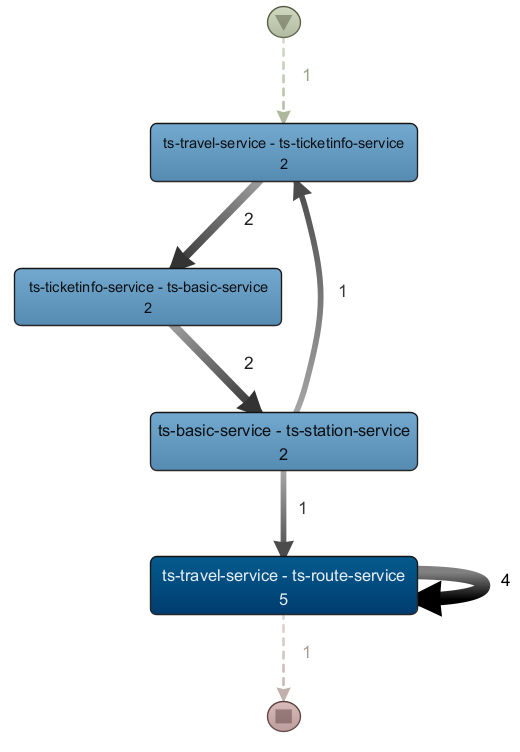
\includegraphics[width=8cm]{RACS2022_Latex_Template/img/bpr.png}
% % \vespaço{-0,4cm}
% \caption{Reconstrução do processo de negócios
% \\(Os números nas setas indicam o número de vezes que um determinado caminho é seguido. Os números nos objetos indicam o número de vezes que um determinado serviço foi chamado)
% }
% % \vespaço{-0,7cm}
% \label{fig:processo de negócios}
% \end{figura}

% Figura \ref{fig:processo de negócios} mostra a reconstrução para um caso de uso único. Observando as interações do serviço, podemos ver que 5 serviços diferentes são chamados. O teste começa com uma chamada para o serviço de viagens, que faz uma chamada de acompanhamento para o ticketinfo-service, que liga para o serviço básico. Usando as frequências de chamada, podemos ver que outra chamada é feita para o serviço de viagens e que esse ciclo se repete. Em seguida, são feitas 5 chamadas finais para o serviço de viagem, que chama o serviço de rota.

% Podemos determinar os serviços pai com base em quais serviços não são chamados por outros. Neste caso, ts-travel-service é o microsserviço que está sendo chamado diretamente pelo teste, e chama os demais microsserviços, que continuam chamando outros serviços para completar o caso de uso. Agora, podemos verificar o teste vendo que ele faz as chamadas especificadas no rastreamento. Todos podem ser encontrados no pacote Zenodo \cite{zenodo_benchmark}.

\section{Referência proposta}
\label{sec:proposto}

\todo[inline]{Sheldon (6/1): Devemos encurtar algumas das coisas introdutórias para o benchmark e focar principalmente em nossas definições dos três componentes de nosso benchmark?}

Com nosso estudo de caso, fornecemos à comunidade um benchmark de teste dos sistemas de microsserviços que avaliamos. A criação de um benchmark de teste permite uma maneira fácil de mostrar à comunidade como os sistemas respondem a uma variedade de testes diferentes. Além disso, eles podem usar o benchmark para simular o sistema usado para realizar análises dinâmicas de sistemas, avaliações de segurança, resiliência ou testes de escala.

Uma chave para testar benchmarks é que eles são repetíveis. Pode servir como ponto de referência para comparar outros produtos e serviços. Esses benchmarks também podem ser usados para comparar os lançamentos de software passados, presentes e futuros com seus respectivos benchmarks. Uma clara evolução dos resultados do software pode ser rastreada usando esses benchmarks.

% Como estamos nos concentrando em testes funcionais e de carga para nosso estudo de caso, nosso benchmark de teste está centrado na avaliação do tempo de resposta das ações, na interação da interface do usuário e na funcionalidade geral do sistema.

% O teste de funcionalidade considera o sistema como uma caixa preta e desconhece a decomposição interna para microsserviços, que muitas vezes reflete a visão do usuário. O benchmark de teste de interface do usuário (baseado na web) ajuda a garantir a consistência durante a execução das ações do usuário.

% Os benchmarks de teste de carga ajudam a identificar possíveis pontos de gargalo e lentidão. Isso é importante porque a experiência do usuário pode ser bastante afetada por esses problemas. No entanto, com o teste de carga, podemos considerar o sistema como uma caixa cinza e focar nos endpoints expostos ao middleware.

No geral, existem três componentes principais de benchmark \cite{benchmark_info}.
\begin{itemizar}
     \item 1. ] \textit{Especificações de Carga de Trabalho}: Esta área de um benchmark abrange a determinação do tipo e frequência das solicitações a serem submetidas ao sistema em um determinado teste. Dentro do teste de carga, isso seleciona o número geral de usuários em um determinado período de tempo que o teste será executado. As especificações de carga de trabalho para teste de navegador da Web envolvem a avaliação da paralelização de testes.
    
     \item[2. ] \textit{Especificações de métricas}: Este componente centra-se em determinar qual elemento específico de um determinado teste será usado para avaliação. Essas métricas podem ser simplesmente se o teste geral foi aprovado ou reprovado, o tempo de resposta das solicitações, a eficiência dos testes ou alguma outra métrica.
    
     \item[3. ] \textit{Especificações de medição}: O último componente principal de um benchmark de teste é determinar como medir as métricas especificadas para avaliar os resultados. Essa determinação também é indicada como os critérios do Acordo de Nível de Serviço (SLA). Isso pode envolver um determinado limite para o número de solicitações aprovadas em um determinado tempo de resposta ou se todos os testes foram aprovados ou não.
    
\end{itemizar}

No teste de carga, é importante manter a carga o mais realista possível para a carga de trabalho normal do sistema. Isso dará uma melhor compreensão de como o sistema reage em circunstâncias típicas. Infelizmente, há poucos dados sobre a quantidade normal de usuários que acessam esses sistemas de microsserviços. Com isso em mente, decidimos testar uma variedade de cargas diferentes, começando com um teste básico baixo de 100 usuários e indo até 5.000 usuários como nosso máximo. Isso ajudou a definir nossa especificação de carga de trabalho para 100 usuários, 500 usuários, 1.000 usuários, 2.500 usuários e 5.000 usuários.

Para manter a consistência da execução do teste, essas cargas são executadas em um período de 30 segundos. As especificações métricas que utilizamos para medir os resultados foram o tempo de resposta de cada requisição. A cada teste, conseguimos dividir o número de respostas que levaram menos de 800ms, entre 800ms e 1200ms e maiores que 1200ms.

Verificou-se que o tempo de resposta mais preferido para os sistemas é de 0,1 segundos ou 100ms. No entanto, o limite máximo de tempo de resposta aceitável é normalmente definido em 1 segundo ou 1.000 ms \cite{hamilton2023response}. Com isso em mente, decidimos definir nosso tempo de resposta aceitável em 0,8 segundos ou 800 ms, uma vez que se prestava bem à ferramenta de teste que usamos. Isso nos leva a determinar que a especificação das medições para os testes de carga seria a porcentagem de requisições que levaram mais de 800ms para serem concluídas. Optamos por utilizar uma porcentagem ao invés de um número específico para auxiliar melhor esta escala métrica em testes com diferentes cargas. Decidimos que um determinado caso de uso foi capaz de lidar com a carga específica se a porcentagem de solicitações que levaram mais de 800ms for menor que 20\%

%\todo[inline]{Cerny TODO: O critério de regressão é bom?}

Ao escrever testes de regressão para um navegador da Web, é importante tentar fazer com que os testes sejam executados da maneira mais eficiente possível para reduzir o tempo de execução. Como os testes serão executados muitas vezes após alterações ou atualizações no código, eles precisam ter um tempo de execução baixo. Para diminuir o tempo de execução, utilizamos o framework TestNG para paralelizar os testes do Selenium para os microsserviços. Decidimos dedicar cada teste à sua própria thread para reduzir ao máximo o tempo de teste.

Agrupamos nossos testes de regressão por serviço, de modo que cada teste incluiria muitas afirmações sobre as várias partes do sistema fornecido. Usamos as afirmações individuais como nossas especificações métricas. As afirmações individuais e ações tomadas durante o curso do teste são o fator determinante para a avaliação.

Para nossos testes de regressão, medimos as afirmações determinando se um teste coletivo passou ou falhou. Se uma das asserções em um teste falhar, isso fará com que todo o teste falhe. Medimos o sucesso do teste apenas se o teste inteiro passou ou falhou.

Após a conclusão, se nosso estudo de caso resultar em benchmark de teste para sistemas de microsserviços específicos, compartilharemos nosso conjunto de testes com o Zenodo \cite{zenodo_benchmark}. Este site é um repositório aberto para os membros da comunidade compartilharem uma variedade de recursos, como artigos de pesquisa, conjuntos de dados, software de pesquisa e relatórios.
%
Compartilhamos o benchmark de teste para permitir que outros pesquisadores e engenheiros da indústria de teste na comunidade interessados em rastrear os resultados dos testes os expandam.

% \section{Ameaças à Validade}

% %\todo[inline]{Cerny TODO: atualizamos esta seção}

% Os estudos de caso podem muitas vezes estar a par de vários tipos de ameaças à validade. Enquanto trabalhávamos neste estudo de caso, tentamos eliminar o efeito que essas ameaças têm sobre o resultado do estudo. Nesta seção, discutiremos dois tipos principais de ameaças de validade: validade externa e validade interna.

% \subsection{Validade Externa}

% A validade externa envolve a compreensão de como os achados de um determinado estudo podem ser generalizados para outras situações. Determinar até que ponto esses resultados podem ser aplicados a um contexto mais amplo é um tópico importante. Um objetivo central da pesquisa e dos estudos de caso é entender qual conhecimento ela produz sobre outras situações semelhantes.

% A validade externa se aplica a este estudo de caso principalmente devido à análise de como os resultados dos testes desses dois sistemas de microsserviços bem estabelecidos se aplicariam a outros sistemas. Para nosso estudo de caso, escolhemos os sistemas de referência devido à ampla gama de serviços fornecidos por esses sistemas de microsserviços. Isso ajuda a aumentar a capacidade de generalizar nossos resultados e conclusões para outros sistemas com uso semelhante.

% Uma ameaça principal à validade externa nesse caso é que cada sistema de microsserviço implementa pontos de extremidade ligeiramente diferentes uns dos outros. Portanto, pode ser difícil supor que cada sistema responderá da mesma maneira a várias quantidades de entrada. No entanto, nossos testes não são afetados diretamente pela forma como os endpoints são implementados, pois os testes estão apenas observando a resposta e a solicitação dos endpoints.

% Ao focar nossos testes nos endpoints e no fluxo geral do sistema, tentamos mitigar o efeito que diferentes linguagens e técnicas de programação teriam em nossos resultados. Nosso estudo de caso se concentra principalmente nas partes de nível superior do código, criando um objetivo mais generalizado para nossos testes.
% %https://www.scribbr.com/methodology/external-validity/#:~:text=There%20are%20seven%20threats%20to,aptitude%2D treatment%20and%20situation%20effect.

% \subsection{Validade Interna}

% A validade interna refere-se à medida em que os resultados de um determinado estudo não podem ser explicados por outros fatores. Esse tipo de validade garante que haja uma ligação entre a causa e o efeito do estudo. Isso garante que as conclusões desse relacionamento sejam críveis e confiáveis.

% Para lidar com essa ameaça, verificamos que os testes estavam completos e funcionando por meio da análise de outros membros do estudo. Isso garante que os resultados sejam consistentes. O código de referência, incluindo os testes e casos de uso encontrados, são acessíveis publicamente e podem ser validados.

% Semelhante à discussão anterior sobre validade externa, muitas das ameaças são mitigadas devido aos testes serem os mesmos em diferentes execuções. Enquanto a conexão com o sistema de microsserviço permanecer estável, os testes funcionarão sem viés interno. A ameaça de mudanças em testes repetidos e maturação não afetará este estudo de caso, pois os testes são consistentes e estáveis ao longo de várias execuções.
% %https://www.scribbr.com/methodology/internal-validity/#:~:text=What%20are%20threats%20to%20internal,mean%2C%20social%20interaction%20and%20attrition.

\section{Conclusão}
\label{sec:conclusão}
%\todo[inline]{Cerny TODO: isso será suficiente como conclusão?}

Este artigo apresenta um novo conjunto de testes que pode ser efetivamente usado como benchmark para pesquisas sobre teste de software em sistemas baseados em microsserviços. Nossa abordagem considerou tanto o teste de regressão funcional quanto o teste de carga. Selecionamos dois sistemas de microsserviços bem estabelecidos para criar um benchmark de teste para fornecer à comunidade. Esses sistemas de referência foram Train-Ticket e eShopOnContainers.

Nossa abordagem dupla para avaliar o desempenho dos sistemas de microsserviço ajuda a destacar as principais áreas de falha nesses sistemas. O aspecto do teste de carga de nosso estudo de caso destaca áreas dentro dos endpoints que podem causar um gargalo ou falha devido a diferentes quantidades de carga. Compreender como o sistema responde a várias quantidades de carga pode ajudar os designers a entender as áreas para ajudar a melhorar a experiência do usuário. Nosso segundo aspecto de teste envolve a análise do sistema usando testes de regressão funcional. Especificamente dentro dessa abordagem, usamos testes automatizados do sistema da Web para garantir que o sistema seja exibido de maneira correta e consistente em vários ambientes de navegador.

A contribuição deste trabalho para a comunidade é (1) fornecer um exemplo de código aberto de testes de regressão funcional automatizados e testes de carga para sistemas de microsserviços, pois os exemplos publicados anteriormente não são suficientes e (2) produzir um conjunto inicial de testes para um benchmark proposto de sistemas de microsserviços bem estabelecidos.%, e (3) para demonstrar como uma reconstrução de processo de negócios pode ser usada como uma forma de validar cenários de teste.

%\begin{itemize}
%    \item 1. ] para dar um exemplo de código aberto de uma boa configuração de testes funcionais e de carga automatizados para sistemas de microsserviços, pois os exemplos publicados anteriormente não são suficientes
    
% \item[2. ] para fornecer um conjunto inicial de testes abrangentes para um benchmark proposto de sistemas de microsserviços bem estabelecidos
    
% \item[3. ] para mostrar como uma reconstrução de processo de negócios pode ser usada como uma forma de validar cenários de teste.
    
%\end{itemizar}

% Nosso benchmark proposto pode ser útil para a comunidade acadêmica, especialmente para entender como os sistemas de microsserviços podem ser avaliados com base em seu desempenho.

% \begin{acks}
% \hl{FIXME} Este material é baseado no trabalho apoiado por Cerny
% \end{acks}